\section{Data Integration and Analysis System}
\label{se:dias}

\acrfull{dias} \cite{Kawasaki2018DataReduction} collects and archives data from satellites, weather stations, numerical forecasting models, and climate projection models. Once these data integrate into useful geographic information, DIAS generates results for managing global environmental problems and natural disasters \cite{Kawasaki2018DataReduction}. The \acrshort{dias} can assimilate weather data from multiple data sources with different data formats. After successfully storing the data, it generates results which can be used for different kinds of purposes by other parties.

\begin{figure}[htp]
    \centering
    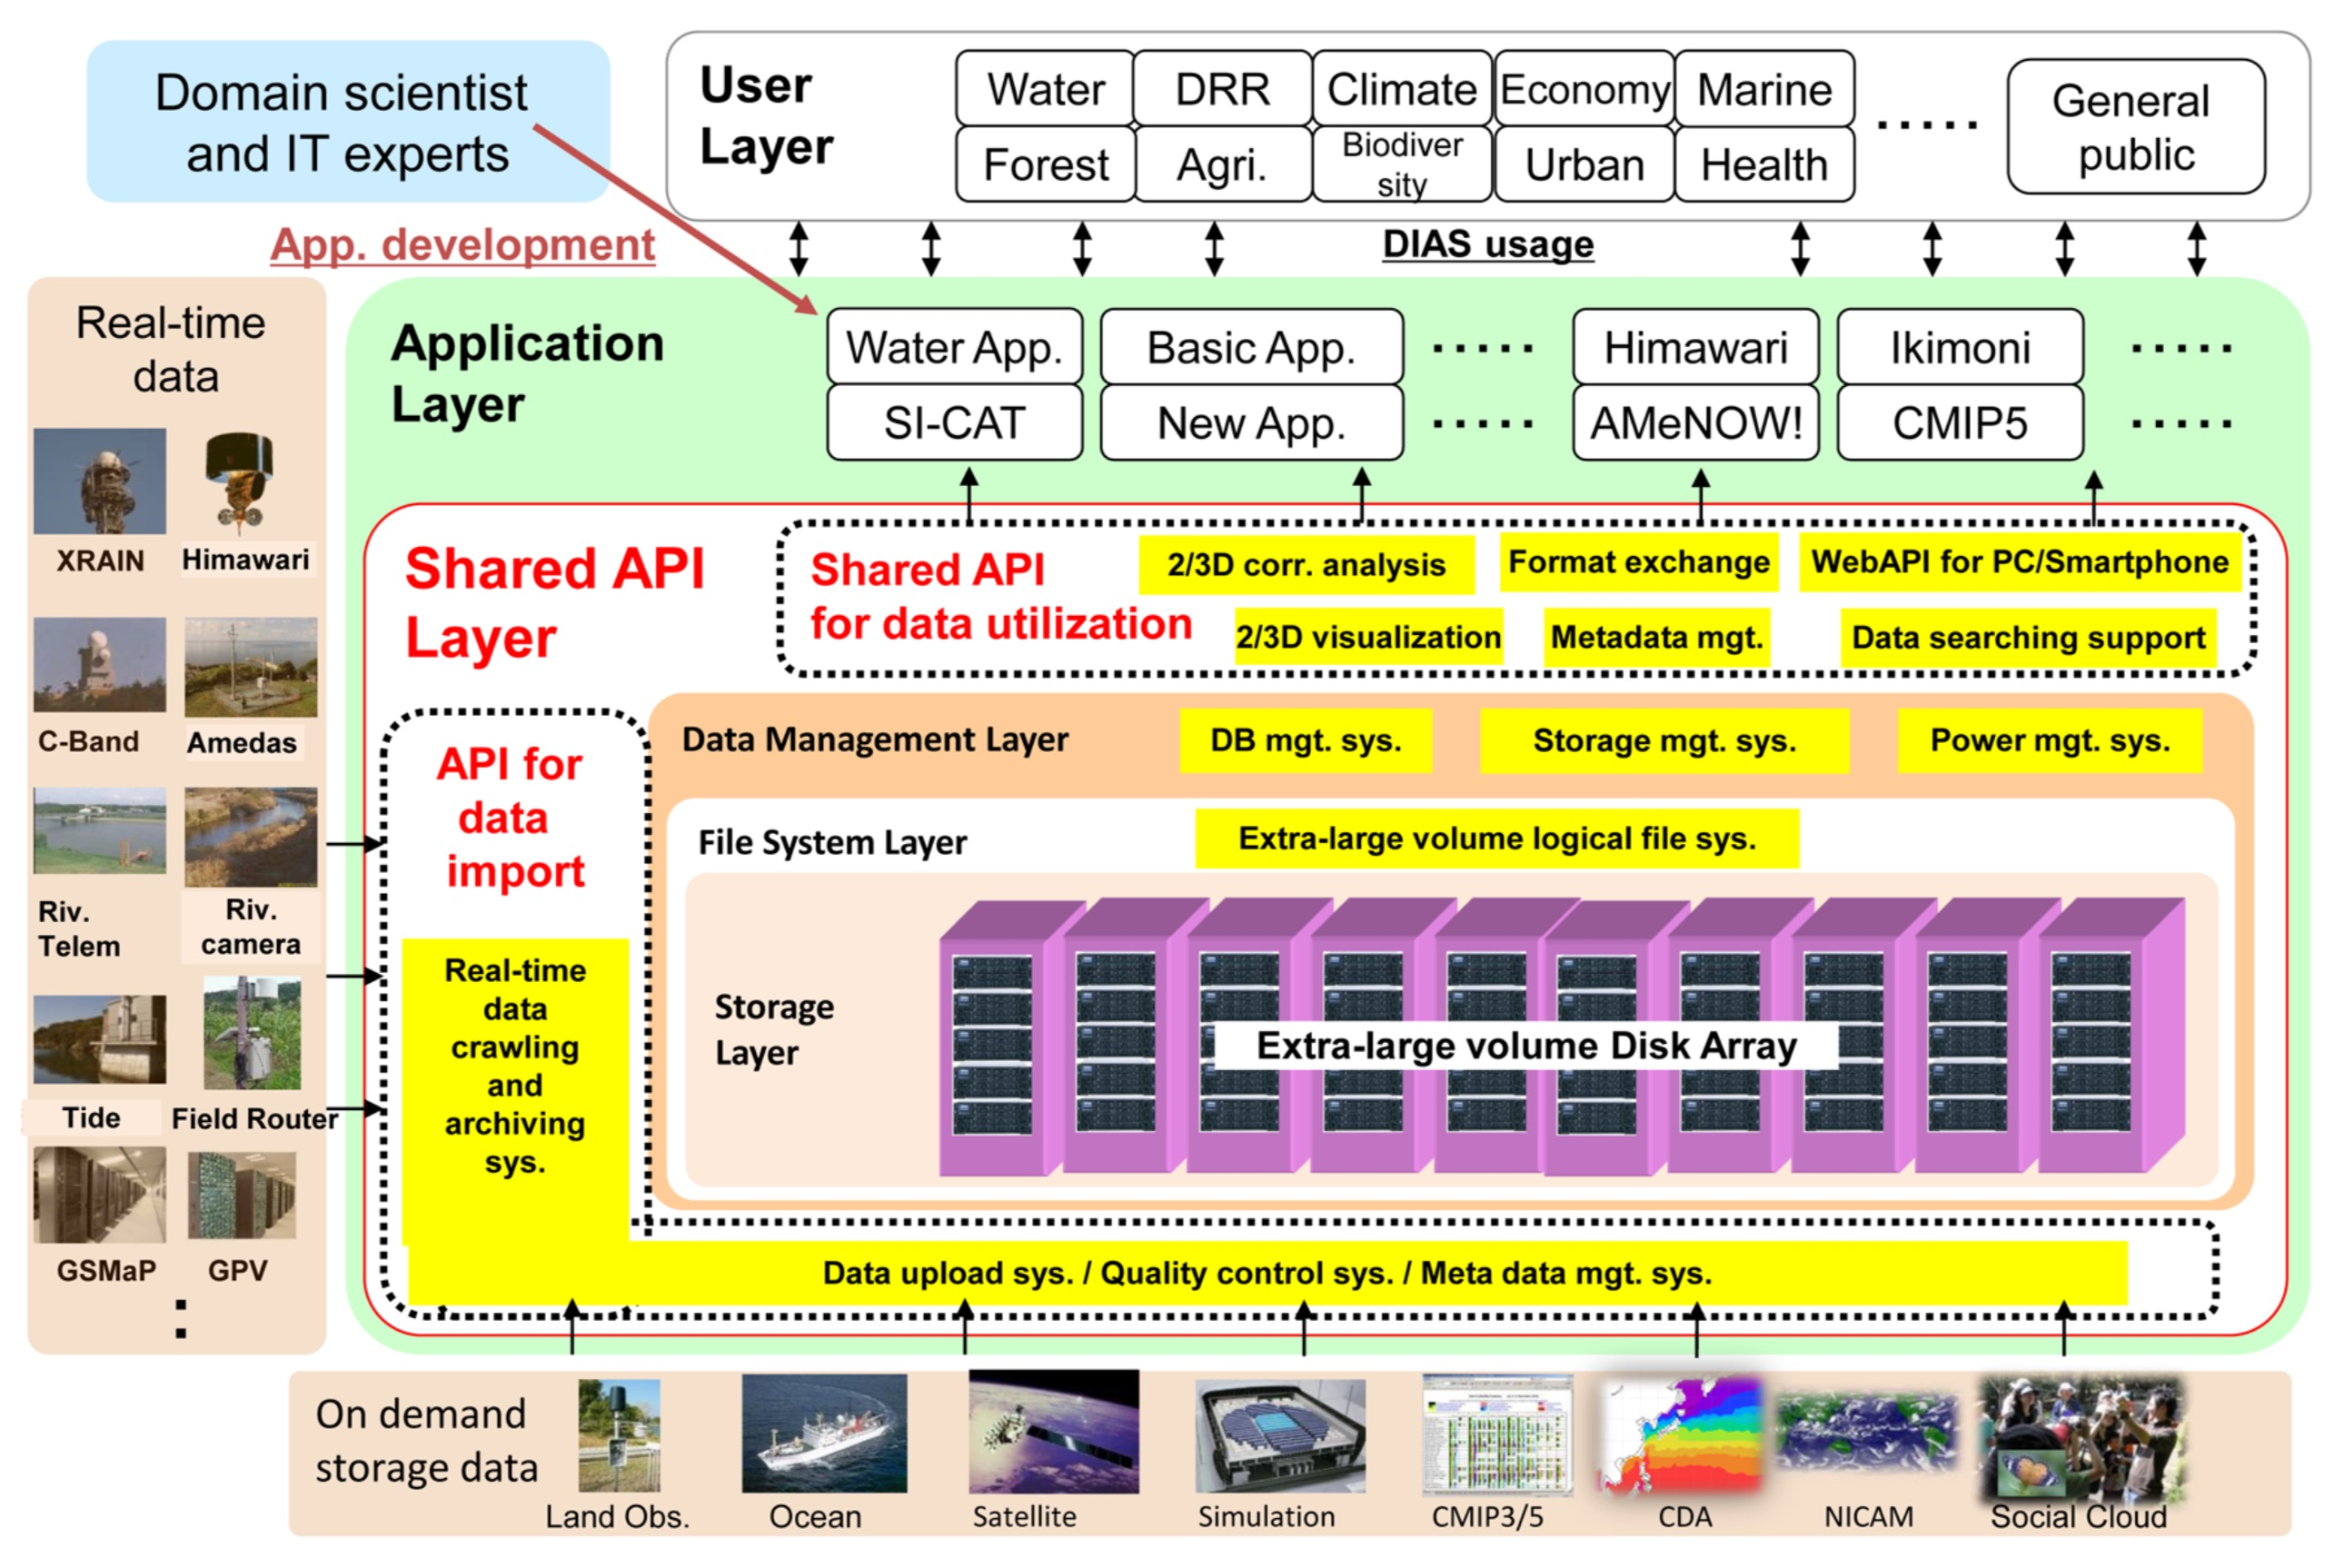
\includegraphics[width=1\textwidth]{lit/other/dias_common_base_application_platform.jpg}
    \caption[DIAS’s common base application platform.]{DIAS’s common base application platform \cite{Kawasaki2018DataReduction}.}
    \label{fi:dias_common_platform}
\end{figure}

The data storing mechanism is similar to the other systems discussed above. The DIAS provides an API to import the data and store them in a large array of storage after converting to the required data format. The APIs work to convert or reformat data into manageable forms and are useful for creating the DIAS storage archive. The DIAS's API contains various tools, including the real-time data exploration and archiving system, the data download system, the quality control system, and the metadata management system \cite{Kawasaki2018DataReduction}. To store on the large volume of disk space, it converts the data via a provided set of APIs. The above concept is similar to Delft-FEWS's open data model approach, but it has extra-large storage volume and a database management system which abstract for the upper layer to access the data. Further, the DIAS contains additional tools that provide the functionality of quality control of the data and metadata management, which is similar to some of the services in LEAD.

As shown in \cref{fi:dias_common_platform}, it offers an application layer that allows scientists to work on research tasks and to develop specific tools and applications by collaborating with IT experts \cite{Kawasaki2018DataReduction}. Once the data is stored on the \acrshort{dias} system, it shares those data via the shared API layer and allows users to remote access to the data and easy integration via the APIs.


%%%%%%%%%%%%%%%%%%%%%%%%%%%%%%%%%%%%%%%%%%%%%%%%%%%%%%%%%%%%%%%%%%%%%%%%%%%%%%%%
\section{Meteorological Assimilation Data Ingest System}
\label{se:madis}

\acrfull{madis} \cite{Macdermaid2005ArchitectureP2.39} is a data integration and assimilation system as the name implies that collects data from dozens of suppliers, then checks the quality of the data and saves it in \acrshort{netCDF} format. Later, users can access the data with the support of the different types of data access protocols.

\begin{figure}[htp]
    \centering
    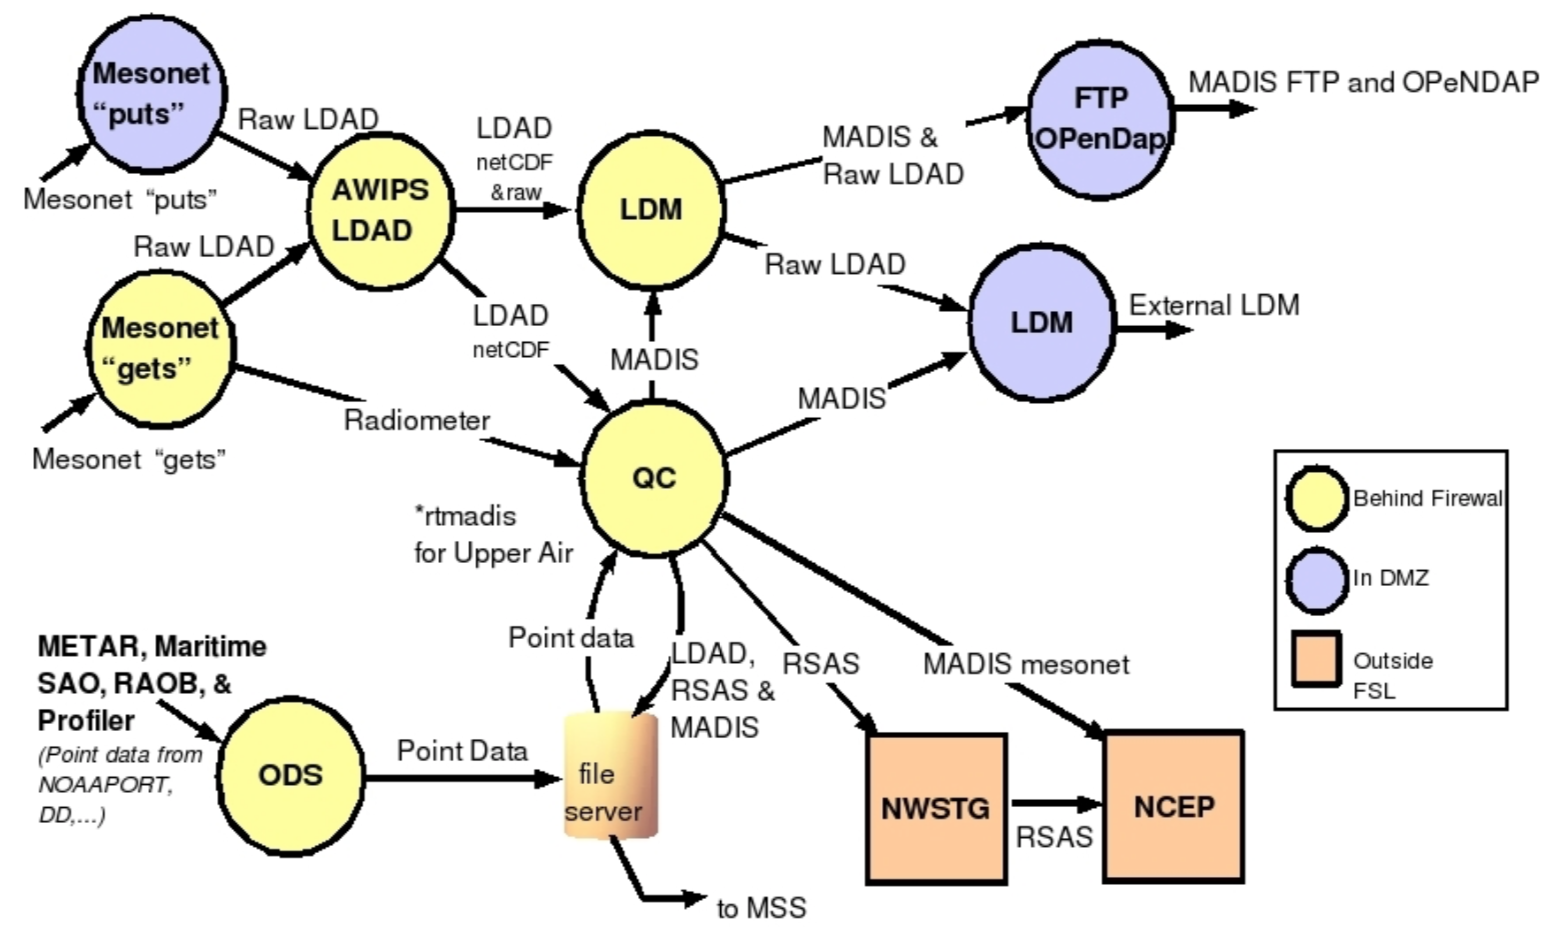
\includegraphics[width=1\textwidth]{lit/other/madis_flow.png}
    \caption[\acrshort{madis} data flow]{\acrshort{madis} data flow \cite{Macdermaid2005ArchitectureP2.39}.}
    \label{fi:madis_flow}
\end{figure}

MADIS contains a distributed architecture for data acquisition, processing, and distribution functions. Besides, the MADIS was developed based on the distributed architectural patterns available at the time of implementation. The various functional hosts have been paired using Linux High Availability (HA) to provide automated failover in the event of a system failure. It uses several methods for data dissemination such as FTP, Local Data Manager (LDM), and the Web OPeNDAP (OPen source project for Network Data Access Protocol) \cite{Macdermaid2005ArchitectureP2.39}. It uses functional calls like Remote Procedure Call (RPC) to invoke among the cluster of nodes. In \cref{fi:madis_flow}, the data is transported from the input and preprocessing systems to the central computer systems and then to other hosts for storage and distribution \cite{Macdermaid2005ArchitectureP2.39}. To get high availability, it has added some updates to its architecture, as mentioned in the paper.

Based on the above statements, we can conclude that these kinds of functionalities are available at the modern cloud computing tools out of the box, and those tools are providing the scalability and high availability. Using those tools, it is possible to implement such a system with less effort and high confidence.

The MADIS regularly acquires mesonet data from dozens of network providers representing more than 14,000 stations, and the system translates into more than 30,000 station reports every hour. Different systems that work inside and outside the firewall collect the data. The collected data is sent to the data server of the Advanced Weather-Interactive Processing System (AWIPS) of the central installation for processing and conversion to a common data format, NetCDF. The NetCDF files are then transferred to MADIS compute nodes \cite{Macdermaid2005ArchitectureP2.39}. After reading the statistics of the MADIS system, I realized the paper is a useful reference for system architecture design and its performance testing. When compared to the Delft-FEWS, the MADIS also converts the assimilated data into netCDF format. After converting to netCDF format, the netCDF files are transferred to the compute nodes and accessible via OPeNDAP. Many of these computers are configured using Linux clustering with high availability \cite{Macdermaid2005ArchitectureP2.39}.

Some of the MADIS data is considered to be the property of the supplier, and data access should be provided based on the authorization. To address the issue, MADIS data is divided into six different versions, depending on the access level authorized by the data provider \cite{Macdermaid2005ArchitectureP2.39}. When compared to Delft-FEWS, MADIS provides data assimilation with control-based access to the data.

%%%%%%%%%%%%%%%%%%%%%%%%%%%%%%%%%%%%%%%%%%%%%%%%%%%%%%%%%%%%%%%%%%%%%%%%%%%%%%%%
\section{Meta Scientific Modeling}
\label{se:msm}

\acrfull{msm} framework developed an open system architecture that consists of open-data concept to access heterogeneous data sources via data agents, and open-model concept to allow management of individual model via model agents. Even though other systems like \acrshort{fews} provide these features, they do not provide decentralized model execution and data integration. Specifically, this framework provides a graphical user interface for workflow creation similar to \acrshort{lead}, rather than providing a configuration-based workflow system as in \acrshort{fews}. \acrshort{msm} tries to effectively address the drawbacks of the existing modeling systems by providing features such as an independent open-source and graphical-based workflow engine, facilitating  users to obtain data directly from popular sources, decentralized model administration by modelers, and enables models to be freely connected with each other in the \acrshort{msm} framework. However, in our research, we focus on data ingress and egress aspects than the workflow engine.

\cref{fi:msm_architecture} shows the \acrshort{msm} framework from a top-level design point of view, and it is mainly composed of the \acrshort{msm} core which is an interface with the workflow engine, data agents, and model agents. Thus, the \acrshort{msm} core can lead to a bottleneck and a single point of failure in critical situations. The \acrshort{msm} core also controls all other components, and by using corresponding model agents and data agents allows it to connect with external models and remote data sources. The \acrshort{msm} core is connected to the workflow engine and provides the end-user with all workflow control capabilities, and it contains data persistence services that can be used by all \acrshort{msm} components. Another drawback is, implementing new data agents and model agents are programming language dependent. To implement model and data agents, users need to inherit \acrshort{msm} classes in the provided language. Then the users need to upload the code into a folder (not a containerized mechanism, or continuous service deployments).

\begin{figure}[htp]
    \centering
    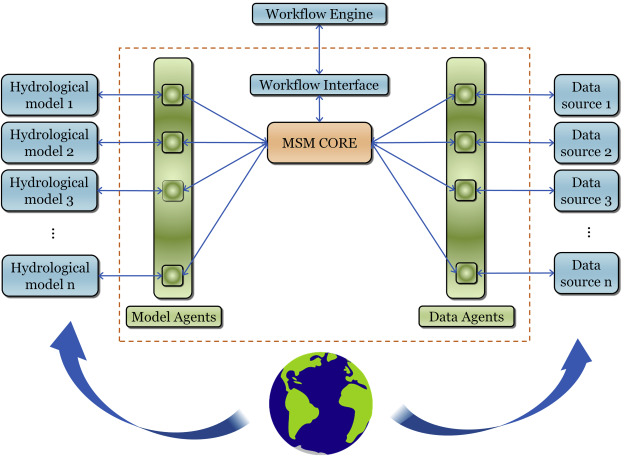
\includegraphics[width=0.99\textwidth]{lit/other/msm_architecture.jpg}
    \caption[The top-level design and overall architecture of \acrshort{msm} system]{The top-level design and overall architecture of \acrshort{msm} system \cite{Salas2020AnApplication}.}
    \label{fi:msm_architecture}
\end{figure}

The open-data architecture of \acrshort{msm} is used to access multiple and heterogeneous external data sources. The users are able to integrate data from any source via data agents, but the data agents are depending on inheriting a generic class to do so. Which means there is a language dependency. The open model architecture allows users to develop and deploy their own model via model agents. Here users also have to use a generic agent provided by the \acrshort{msm} framework, but the models can be implemented independently. Users can deploy new model agents by copy-pasting the source code to a specific folder, but it is possible to run the models written in languages such as C, C++, FORTRAN, Python, and Java. The model execution follows a flow similar to the \acrshort{fews} model adapter with a prepared input file, execute the model, and processing output files. The \acrshort{msm} framework has a data management layer that stores the data as an in memory and local data caching, featuring a non-relational database scheme that supports high throughput. It stores particular timeseries data as msmDataSets, and creates a unique identifier for each msmDataSet. The msmDataSets storage framework contains the time-steps. Each time-step contains a reference to the msmDataSet it belongs to, and a document (the data-oriented structure) with a 2D image.

While the authors presented a use case of using the \acrshort{msm} system, detailed evaluation regarding its performance was not given. Nevertheless, it demonstrates the usefulness and effectiveness of the framework in various aspects of scientific modeling activities. The \acrshort{msm} has only been fully tested on Windows 10 operating system, which means the framework has some operating system dependency. Further, details on how it parallellize data agents, model agents, and the \acrshort{msm} core are not presented. Even though the authors mentioned that \acrshort{msm} follows a decentralized agents approach, it seems to have a monolithic distributed architecture based on the available data. 


%%%%%%%%%%%%%%%%%%%%%%%%%%%%%%%%%%%%%%%%%%%%%%%%%%%%%%%%%%%%%%%%%%%%%%%%%%%%%%%%
\section{Summary}
\label{se:lit_summary}

We presented several related works on WDIA system implementations such as \acrshort{fews}, \acrshort{lead}, \acrshort{dias}, \acrshort{madis}, and \acrshort{msm}. During our research, one of the significant issues that we focused on, store the data ingested from different sources with different formats efficiently. The \acrshort{fews} and \acrshort{madis} are using the netCDF as the common data format to store the data, which is one of the best solutions available with modern technologies as well. Even the \acrshort{lead} and \acrshort{dias} papers are not mentioned directly; those systems are also following a method of having common storage space to store bulk data. The \acrshort{fews}, \acrshort{lead}, and \acrshort{msm} have the capability of handling forecasting workflow, but other systems are mainly focused on providing a weather integration and data management system. The \acrshort{fews} provides a modular approach via its general adapter, and according to the \acrshort{soa} architecture of \acrshort{lead} provides the same functionality via services.

Above WDIA systems are developed with the contributions from lots of researchers, and were implemented specifically to address issues like natural disasters. A use case such as \acrshort{curw}, a given WDIA system requires to remodel the systems and define the forecasting flows to support the country-specific requirements. Even some of the systems try to follow a generic approach to integrate new modules, but it is challenging to deploy modules for a closed source or proprietary software. Further, most of the systems depend on the underline software platform and do not support more resource-efficient and highly-scalable technologies such as cloud computing.
